%!TEX root = ../template.tex
%%%%%%%%%%%%%%%%%%%%%%%%%%%%%%%%%%%%%%%%%%%%%%%%%%%%%%%%%%%%%%%%%%%%
%% chapterNextSteps.tex
%% NOVA thesis document file
%%
%% Chapter with the template manual
%%%%%%%%%%%%%%%%%%%%%%%%%%%%%%%%%%%%%%%%%%%%%%%%%%%%%%%%%%%%%%%%%%%%

\typeout{NT FILE chapterNextSteps.tex}%

\chapter{Next Steps}
\label{cha:next_steps}

\section{Calendar}
\label{sec:Calendar}

As we can see bellow in the calendar this work is several steps behind the initial plan. The main reason for this is the lack of time to dedicate to this work.
 Right now the ideas are scattered to finish the state of the art, so will need more time to pass it to the document citing the sources and making the necessary connections.


\begin{figure}[htbp]
    \centering
    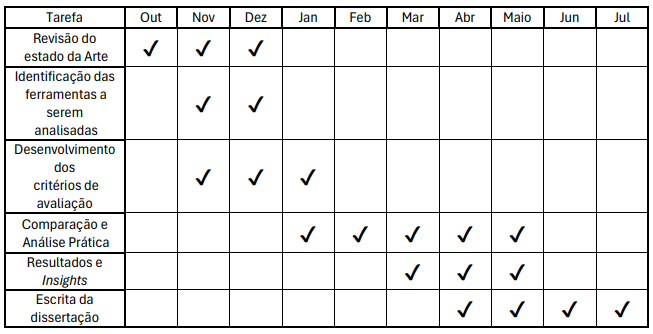
\includegraphics[width=0.7\linewidth]{calendario}%
    \caption{Calendar}
    \label{fig:calendar}
\end{figure}

